% #################################################
% Clause Genome
% #################################################
\documentclass[9pt,academicons]{article}

\usepackage{CADA}
\usepackage{listings}
\lstset{basicstyle=\ttfamily, keywordstyle=\rmfamily\bfseries}




% ####################################
% Add the title of your paper here. Each word is Capitalized! 
% ####################################
\title{Representing Contracts by Clause Genome for Machine Learning Applications}


% #################################################
% This is where your paper begins. 
% #################################################
\begin{document}


% #################################################
% Sets up the beginning of the document (do not modify) 
% #################################################
\maketitle

% % ############################################
% % Here is the fun part. Please enter your:            
% %      Name (First, Middle initial, Last)                  
% %      Your ORCID number replace the "000-0000-1234-5678" part.    
% % ############################################
 \authorSection{
	\anAuthor{Yogesh Kulkarni}{0000-0001-5431-5727}{},
% \anAuthor{First M. Last}{000-0000-1234-5678}{2}, 
%	\anAuthor{First M. Last}{000-0000-1234-5678}{3} 
 }


% % ######################################
% % Here we need your affiliation and contact e-mail. Please edit   
% % affiliation as well as the e-mail fields.                                  
% % ######################################
\affiliationSection{
	\anAffiliation{}{Principal Architect, Icertis Solutions Pvt. Ltd.}{yogesh.kulkarni@icertis.com}
	% \anAffiliation{2}{University of Paris}{author2@uofp.fr}
	% \anAffiliation{3}{Google, Inc.}{author3@google.com}
}


% % ######################################
% % Please decide on who the corresponding author is going to be 
% % and complete the section below                                            
% % ######################################
%\correspondingAuthor{Yogesh Kulkarni}{yogesh.kulkarni@icertis.com}


% ########################################
% Please type in your abstract below after the "\abstract{" part.
% ########################################
\abstract{
Contracts drive large scale commercial transactions. Being a legal document it is binding to all the parties, stakeholders involved. Composition contracts using clauses in an unambiguous manner is key to a good contract design. Contract analysis becomes critical in case of already drafted contract for detecting important clauses, obligations, key attributes, etc. Artificial Intelligence, in form of Machine Learning is being used effectively in some of these critical requirements. Finding similar contracts, grouping them is one such specific example.

Text needs to be converted to numbers in order to be used for Machine Learning applications. Various such vectorization techniques are available, which are primarily statistical in nature and deal with words in the documents. Word vectors are then composed into respective document vectors. This paper proposes vectorization of a higher level abstraction, called clauses, there by bringing domain specific semantic composition into vectorization. Efficacy of the proposed approach has been demonstrated using Similarity and Clustering algorithms.
}


% ########################################
% Please choose at least 3-5 good keywords and list them after the
% "\noindent \textbf{Keywords:}" part.
%
% The DOI part will be edited by us so please do not change that.
% ########################################
\keywords{Clause Genome, Contract Categorization, Representation Learning} 

\doi{10.14733/cadaps.2022.aaa-bbb}


% ################################
% You may now start your paper with an introduction
% ################################

\section{INTRODUCTION}

Contracts are legal documents describing agreements between two or more parties. They have been in practice for ages, evolving in aspects of medium, language and enforcement approaches. Analysis of contracts has become critical for Law firms, companies, governments to assess contents for finding similar documents, extracting important information, etc. Although rule-based approaches have been predominant in this aspect, use of Artificial Intelligence (AI) in form of Machine Learning and Natural Language processing are getting their way into mainstream legal informatics.

Machine Learning approaches need inputs to be in numeric form. For Natural Language Processing (NLP), it becomes imperative 
to convert input (and output, in come cases) to numeric form, such as vectors. Multiple approaches to map words or sentences or document to vectors are available. Some popular ones such as `Bag of Words (BoW)', `Term-Frequency Inverse Document Frequency (Tf-idf)' are typically word frequency based, whereas Word Embeddings such as `Document to Vectors (Doc2Vec)', Glove, `Bidirectional Encoder Representations from Transformers (BERT)' are co-occurrence or contextual in nature. Domain specific embeddings tend to capture some form of semantics due to co-occurrences, ie vectors associated words are closes in embeddings space \cite{Doc2VecSurvey}.

But such word level vectors are too granular to capture higher level domain constructs or abstractions. For example, in case of legal contracts, Doc2Vec would be some sort of composition (say, averaging) of Word2Vec of individual words. This approach loses middle level abstractions such as clauses, ie. Contract is composed of clauses, clauses are composed of words. The middle level abstract actually captures legal-domain semantics.

This paper proposes a novel approach of represent contracts by vector of clauses.
Once documents are converted to list of clause category labels, its a string of labels, similar to biological genome made up of letters such as A, T, C, G. Thus the clause category based representation of contract document is referred to as `Clause Genome'.  They act as signature or short from string of the original document, which can further be vectorized using traditional approaches mentioned above, and then used to Machine Learning algorithms such as Classification, Clustering, Similarity, etc.

% % ##############################################
% % Note how papers are cited. Also, see the references section for more datails.
% % ##############################################


% Significant progress has been made over the past decades with computing
% gradients of objective functions with respect to mesh point perturbation 
% for Computational Fluid Dynamics (CFD) solvers. In particular, the adjoint method
% \cite{pironneau, jameson88aerodynamic, econom15su2,stueck12fresco,jones11mgopt}
% allows to compute these gradients accurately, consistently and with low computational cost.

% \begin{enumerate}[label=\alph*)]
% \item We describe the application of automatic differentiation to a complete CAD
% system and demonstrate the accuracy and efficiency of computation of the shape
% sensitivities. These advances allow us to build gradient-based optimisation
% workflows with the CAD-model being updated inside the optimisation loop. 
% \item We present two alternative approaches that are supported by this
% differentiated CAD kernel, both with their merits and disadvantages. The `explicit' parametrisation is closer to current practice in aeronautics
% and turbo-machinery, but may limit the optimum due to restrictive design spaces.
% The alternative `implicit' parametrisation allows to automatically derive a
% sufficiently rich design space, however may impair convergence to the optimum.
% \end{enumerate}


% A brief introduction to the OCCT differentiation can be found in Sec.~\ref{sec:occtdifferentiation}. Parametrisation of the stator blade with conventional turbomachinery parameters is described in Sec.~\ref{sec:paramtub}. Section \ref{sec:nurbs} describes the necessary ingredients for NURBS-based optimisation including corresponding constraint impositions, followed by results for both approaches in Sec.~\ref{sec:results}.  

\section{RELATED WORK}
\label{sec:litsurvey}
Various schemes are available to convert text to vectors for Machine Learning related applications in the domain of Natural Language Processing. Embeddings come in different forms such as Word  (Word2Vec \cite{mikolov2013distributed}), Sentence (Sent2Vec), Paragraph and Documents (doc2vec). In legal domain, \cite{Chalkidis2017} obtained (pre-trained) word embedding by applying word2vec to an additional unlabeled dataset of about 750,000 contracts.

\section{PROPOSED APPROACH}
\label{sec:proposal}

The proposed approach takes document corpus as input, converts each document into ``Clause Genome'' based intermediate representation, which then taken further into standard Text Classification pipelines such as Vectorization, CLassification model training and results generation. Major steps are enumerated below:

 \begin{itemize}
 \item Data Preparation: Documents, if non-textual format, are converted to text. Text is segmented into paragraphs.
  \item Clause Classification: Each paragraph gets classified into a clause category, thus a document becomes list of clause categories.
\item Symbolization: For each document, using list of clause categories, a ``Clause Genome'' sequence or string is generated. This shortened form now represents the original document in a shortened form.
\item Vectorization: Standard vectorizers like BoW or TfIDF are used on the shortened ``Clause Genome'' string.
\item Application: Genome based vectors can be used in Machine Learning tasks such as Classification and Clustering.
 \end{itemize}

Core steps have been explained in detail, in the following sub sections.

\subsection{Symbolization}
\label{subsec:symbolization}

Typical Master Services agreement will have about 70-100 categories of clauses. Machine Learning based approaches such as Support Vector Machines, Naive Bayes, Neural Networks, can be used to build a classifier. 

After `Data Preparation'' and `Clause Classification' phases, each document is in the form of list of clause categories in it, while maintaining the order of the clause sequence. Each category is mapped to a symbol or label. It can be letters like `a','b','c', etc. But to accommodated large number of categorizes, labeling scheme as `c1','c2', \ldots is used. Sample symbolization map is shown below:

\begin{lstlisting}[language=Python, basicstyle=\footnotesize ]
clause_cateory_to_symbol_map ={ 
"acceptance":"c1", 
"publicity":"c2", 
"amendment":"c3", 
:
"intellectual property rights":"c9", 
"penalties/remedies":"c10", 
"business continuity":"c11", 
:
"payment terms":"c24", 
"force majeure":"c25", 
"governing law":"c26", 
:
"quality control":"c60", 
"preamble":"c61", 
:
}
\end{lstlisting}

For Sample documents like \lstinline|MSA_1| and \lstinline|MSA_2|, the clause genomes look like:
\begin{lstlisting}[language=Python, basicstyle=\footnotesize ]
MSA_1 =  ``c61 c53 c3 c40 c23 c7 c8 c40 c8 c1 c40 c40 c1 c20 c24 c24 c47 c24 c24 c50 c7 c7 c7''
MSA_2 =  ``c61 c61 c48 c48 c8 c34 c40 c40 c8 c24 c47 c1  c49 c14 c29 c2 c30 c24 c30 c9 c53''
\end{lstlisting}

Note that both seem to have started with similar clause category, "c61", and thats obviously "preamble". Pictorially they would look as in Fig. \ref{fig:docclausegenome}:

 \begin{figure}[h!]
 \begin{center}
  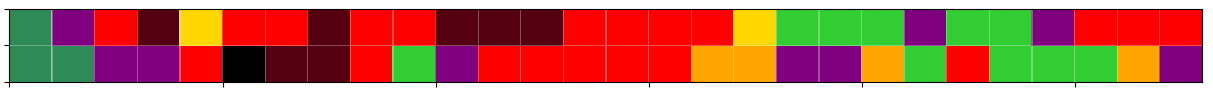
\includegraphics[width=\textwidth,keepaspectratio]{img/two_genomes.png}
  \caption{Graphical representation of document clause genomes}
  \label{fig:docclausegenome}
 \end{center}
 \end{figure}


\subsection{Vectorization}
\label{subsec:vecrtorization}

Instead of the original text, now treat documents are just the genome strings. Use this new content to vectorise them,  tfidf  in the following case as shown in Fig. ref{genomevectors}.

 \begin{figure}[h!]
 \begin{center}
  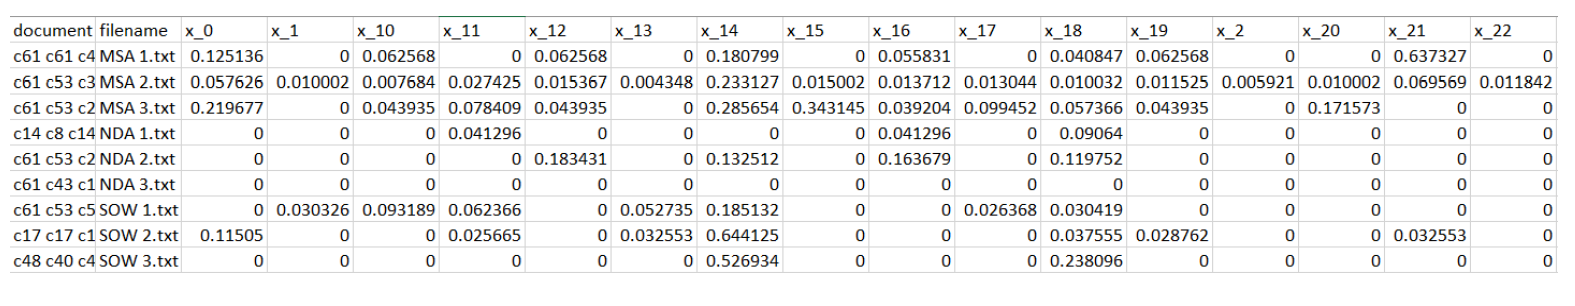
\includegraphics[width=\textwidth]{img/genomevectors.png}
  \caption{Vector representation of document clause genomes}
  \label{fig:genomevectors}
 \end{center}
 \end{figure}


\subsection{Applications}
\label{subsec:application}

Efficacy of the `Clause Genome' based approach for Similarity calculations can be demonstrated by checking two Master Service Agreements (MSA) and then checking between one MSA and one NDA (Non Disclosure Agreement). Results are:

 \begin{itemize}
 \item Cosine Similarity : MSA 1 and MSA 2: 0.734940271290997 
\item Cosine Similarity : MSA 1 and NDA 1: 0.31642358837691426 
\end{itemize}

It can be clearly seen that the similar type of documents have high and dissimilar ones have low similarity score. Meaning, clause genome
representation is quantitatively in agreement with the document language.

Results for checking the efficacy of the `Clause Genome' based approach for Clustering is:

 \begin{figure}[h!]
 \begin{center}
  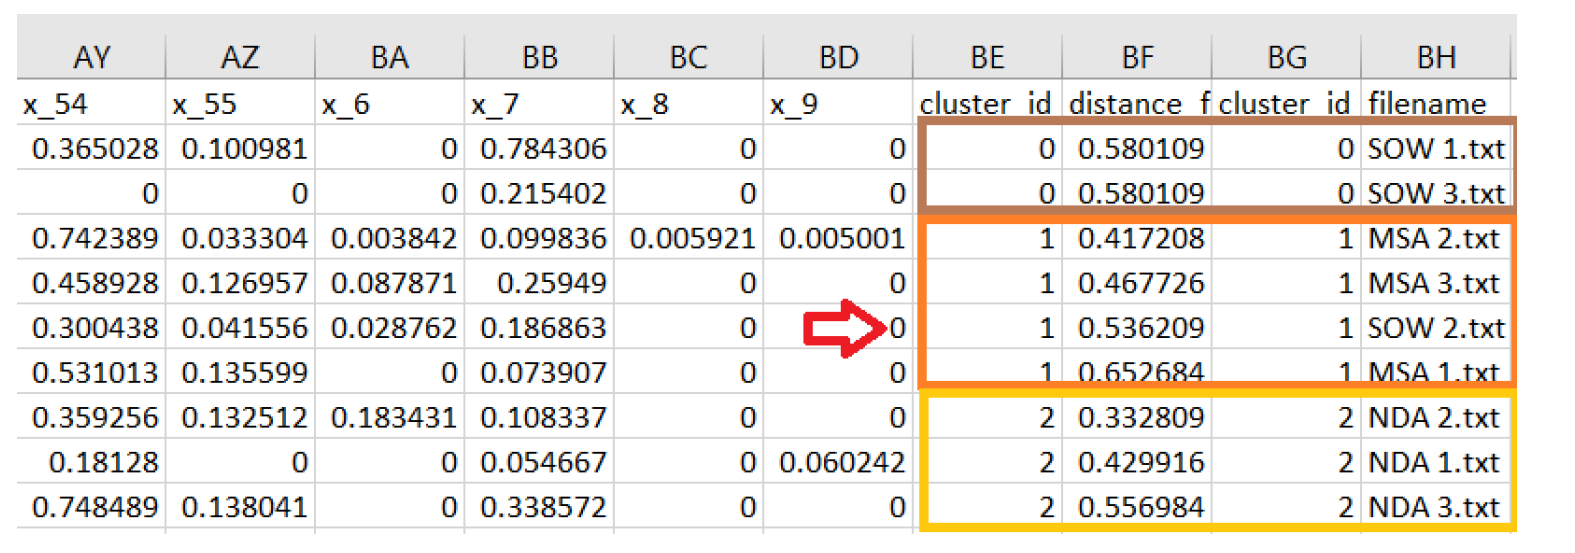
\includegraphics[width=0.6\textwidth]{img/genomeclustering.png}
  \caption{Vector representation of document clause genomes}
  \label{fig:genomeclustering}
 \end{center}
 \end{figure}
 

Barring one misclassification, documents have got correctly segregated into their own type
clusters.

% \begin{figure}
% \centering
% \begin{subfigure}{.5\textwidth}
  % \centering
  % \includegraphics[height=.25\textheight]{img/original-blade.pdf}
  % \caption{Original stator blade shape}
% \end{subfigure}
% \begin{subfigure}{.5\textwidth}
  % \centering
  % \includegraphics[height=.25\textheight]{img/target-blade.pdf}
  % \caption{Perturbed stator blade shape}
% \end{subfigure}
% \caption{CAD optimisation with two stator blades}
% \label{fig:drawtwoblades}
% \end{figure}

% ##############################################
% The sections above show how to include figures and subfigures, how to label
% them, and how to cite them without remembering the figure number. Here 
% are two examples: (1) labeling: "\label{fig:drawtwoblades}" and citing:
% "\ref{fig:drawtwoblades}." LaTeX will do the rest for you.
% ##############################################


% \begin{figure}[h!]
 % \begin{center}
  % \includegraphics[scale=0.35]{img/ADvsFDparam150.png}
  % \caption{Blade sensitivities evaluated by AD (left) and Finite Differences (right)}
  % \label{fig:adfdsensitivity}
 % \end{center}
% \end{figure}

% #############################
% Below is an example of how to include a table.
% #############################

% \begin{table}[h!]
% \centering
% \begin{tabular}{r|ccc}
% & Original sources & AD Forward mode (traceless) & AD Reverse mode (trace-based)\\ \hline
% Avg. time (seconds)& 0.09 & 13.27 & 6.99\\
% Run-time ratio & & 147.44 & 77.67 
% \end{tabular}
% \caption{Timings for initial blade optimization iteration done with original and differentiated (AD) sources}
% \label{tab:computationaltimedifference}
% \end{table}


% \begin{equation}
% \label{eq:cost-func}
% \underset{\alpha}{min} \hspace{0.5em} J(U(X(\alpha)), X(\alpha), \alpha)
% \end{equation}

% \begin{figure}
% \centering
% \begin{minipage}{.5\textwidth}
  % \centering
  % \includegraphics[scale=0.2]{img/sectionCosPic.pdf}
   % \captionof{figure}{Section parameters}
   % \label{fig:2dsection}
 % \end{minipage}%
% \begin{minipage}{.5\textwidth}
  % \centering
 % \includegraphics[scale=0.23]{img/blade2.pdf}
  % \captionof{figure}{Blade skeleton and TE law of evolution in the 3D domain}
  % \label{fig:Blade}
% \end{minipage}
% \end{figure}


\section{CONCLUSIONS}

This paper proposed intermediate level abstraction for representing contract documents, based on clause categories. This approach has following advantages and disadvantages.

 \begin{itemize}
 \item Advantages:
  \begin{itemize}
\item Leverages Contract domain specific higher level abstractions, making it more domain-semantic.
\item Clause genome has lowr space requirements and computationally efficient for further downstream applications.
\item Noise based on individual word frequency is smoothened
\item Order of the clauses is maintained ie document structure is retained
\item Explainability is better for debugging as well as customer trust
\end{itemize}
\item Disadvantages:
 \begin{itemize}
\item Heavily depends on Clause Classifier efficacy
\item Disregards variations within a clause category
\item Loss of word-level information including linguistic structures.
\end{itemize}
\end{itemize}

For future work, multiple word-embedding schemes can be evaluated at, both, clause classification level as well as post-genome vectorization level. Similarly multiple algorithms can be evaluated at, both, clause classification level as well as during usage of the clause-genome based vectors. Best combination can then decided for particular corpus.
%
%\section*{ACKNOWLEDGEMENTS}
%This research is a part of the \ldots


\referenceSection
\bibliographystyle{CADA}
\bibliography{CADA}




\bigskip
\end{document}
